\documentclass[18pt,aspectratio=149]{beamer}
\usepackage[]{bookmark}
\usepackage[utf8]{inputenc}
\usepackage{amsmath}
\usepackage{amsfonts}
\usepackage{amssymb}
\usepackage{tikz}
\usepackage{xcolor}
\usepackage[dutch]{babel}
\usepackage{sansmathaccent}
\usepackage{graphicx}
\usepackage{pgfplots}

\usepackage[style=authoryear,backend=biber]{biblatex}

\addbibresource{bibliography3.bib} 
\pdfmapfile{+sansmathaccent.map}

\title{RMC voor lineaire ODEs}
\author{Isidoor Pinillo Esquivel }
\usetheme{Madrid}

\date{}

\begin{document}

% 1 min
\begin{frame}
    \titlepage
\end{frame}

\section{Introductie}
% 2 min
\begin{frame}
    \frametitle{Introductie}
    \begin{equation}
        y_{t} = A(t)y(t)
        .
    \end{equation}
    Euler:
    \begin{alignat}{2}
        \frac{\tilde{y}(t_{k}+\Delta t)-\tilde{y}(t_{k})}{\Delta t} & = & A(t_{k})                & \tilde{y}(t_{k}) \\
        \tilde{y}(t_{k+1})                                          & = & (I+\Delta t A(t_{k}))   & \tilde{y}(t_{k}) \\
        Y(T_{k+1})                                                  & = & (I+\Delta t A(T_{k+1})) & Y(T_{k})
    \end{alignat}
    $T_{k+1} = T_{k} + \text{Exp}(\Delta t)$, exponentiële verdeelde stappen.
    \begin{equation}
        y(T_{k})=E[Y(T_{k})].
    \end{equation}

\end{frame}

% 1 min
\begin{frame}
    \frametitle{Overzicht}
    \tableofcontents
\end{frame}

% 2 min
\section{Motivatie}
\begin{frame}
    \frametitle{Motivatie}
    Veralgemenen van WoS algoritme van (\cite{sawhney_grid-free_2022})
    naar tijd
    \vspace{-0.25cm}
    \begin{figure}[h!]
        \centering
        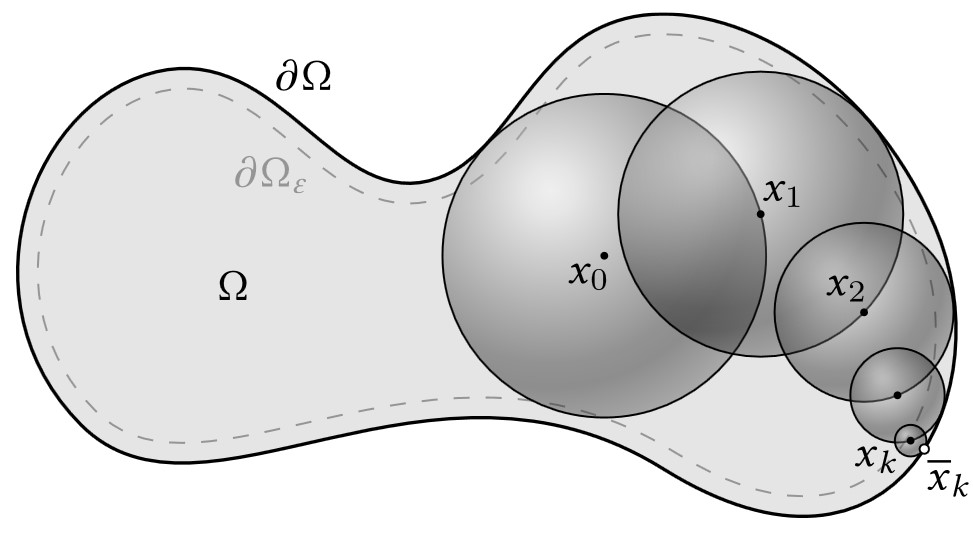
\includegraphics[width=0.6\textwidth]{imgs/Walk_on_Spheres_illustration.jpg}
        \label{fig:Walk_on_Spheres_illustration.jpg}
    \end{figure}
\end{frame}

\section{Monte Carlo}
\begin{frame}
    \frametitle{Monte Carlo}
    \tableofcontentscurrent
\end{frame}

% 2 min
\begin{frame}
    \frametitle{Random sample efficientie van optelling}
    \action<+->{
        Probleem: benader $\bar{x} = \frac{1}{k}\sum_{i=1}^{k} x_{i}$ met $n<<k$ van $x_{i}$'s $\in [0,1]$\\
        (symmetrisch in $x_{i}$) \\
        \vspace{0.2cm}
    }
    \action<+->{
        Vertrouwensinterval kans $=1$  $\sim \frac{k-n}{k}= 1-\frac{n}{k} \approx 1$ \\
        (worst case $\frac{1}{k}$ uit elkaar) \\
        \vspace{0.2cm}
    }
    \action<+->{
        Samplen of termen willekeurig weg laten (Russische roulette)
        \begin{equation}
            \bar{x}  \cong \frac{1}{n}\sum_{i=1}^{n} x_{I_{i}} \cong \frac{1}{k}\sum_{i=1}^{k} B_{i} x_{i}
            .
        \end{equation}
        $\left(E[B_{i}] = 1, P[B_{i}=0]=1-\frac{n}{k}\right)$ \\
        \vspace{0.2cm}
    }
    \action<+->{
        Variantie = RMSE $\sim O\left(\frac{1}{\sqrt{n}}\right)$ en ook vertrouwensintervallen kans $<1$\\
        (CLT of Chebychev's ongelijkheid)\footcitetext{heinrich_optimal_2001}\\
    }

\end{frame}

% 1 min
\begin{frame}
    \frametitle{Optelling algoritmes (plot)}
    \begin{figure}[h!]
        \centering
        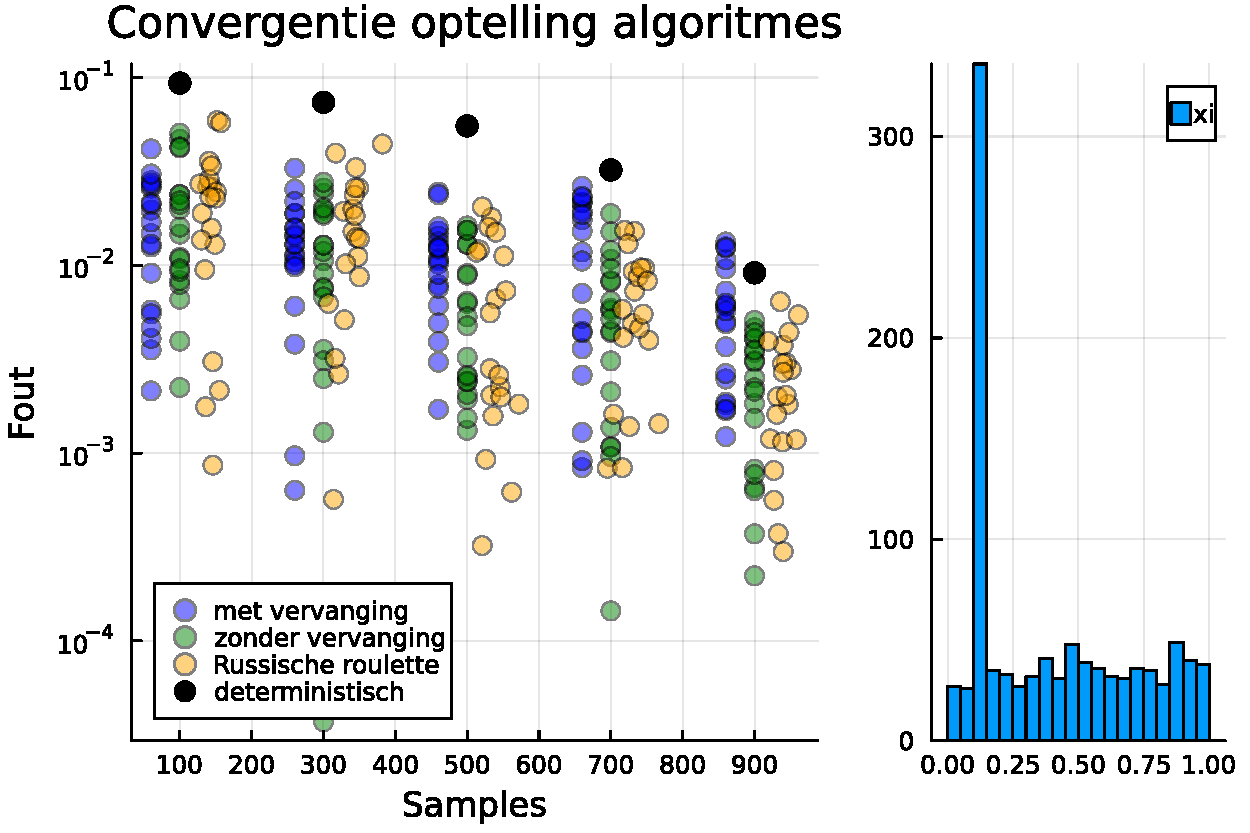
\includegraphics[width=0.8\textwidth]{imgs/convergence_sums.pdf}
        \label{fig:convergentie_optelling}
    \end{figure}
\end{frame}

% 1 min
\begin{frame}
    \frametitle{Monte Carlo integratie}
    Integratie $\approx$ sommatie, integreerbare $f: \mathbb{R} \rightarrow [0,1]$:
    \begin{align}
        \int_{0}^{1} f(s) ds & = E[f(U)]                                 \\
                             & \cong \frac{1}{n} \sum_{j=1}^{n} f(U_{j}) \\
        \text{met } U_{j}    & \sim \text{Uniform}(0,1)
    \end{align}
\end{frame}

\begin{frame}
    \frametitle{Overzicht integratie}
    Beschouw $f:[0,1]^d \rightarrow [0,1]$ $k$-keer Lipschitz-differentieerbaar:
    \begin{equation}
        \int_{[0,1]^d} f(x) dx  .
    \end{equation}
    \pause
    CVMC = Control Variate MC, $+0.5$ orde over DET algoritmes \\
    FFT = Clenshaw-Curtis/Gauss Quadrature.
    \pause
    \begin{table}
        \centering
        \begin{tabular}{lcccc}
                            & $k=-1$ & $0 \le k \le 2$ & $3 \le k \le 5$ & $k>5$ \\
            $d=1$           & MC     & CVMC            & ?               & FFT   \\
            $2 \le d \le 5$ & MC     & CVMC            & CVMC            & ?     \\
            $d>5$           & MC     & MC              & MC              & MC    \\
        \end{tabular}
        \caption{Overzicht integratie algoritmes.}
    \end{table}
\end{frame}

\section{Main Poisson algoritme}

\begin{frame}
    \tableofcontentscurrent
\end{frame}

% 2 min
\begin{frame}
    \frametitle{Main Poisson algoritme}

    \begin{align}
        \action<+->{y_t                              & = A(t) y,  \quad A(t) \text{ meetbaar en } \sup _{t}||A(t)||< \infty  \Leftrightarrow                                                              \\}
        \action<+->{y_t+\sigma y                     & = (\sigma I + A(t)) y \Leftrightarrow                                                                 \\}
        \action<+->{e^{-\sigma t} ( e^{\sigma t}y)_t & = (\sigma I + A(t)) y    \Leftrightarrow                                                               \\}
        \action<+->{y(t)                             & = e^{-\sigma t} y(0) + \int_{0}^{t} e^{(s-t) \sigma} \left(  \left(\sigma I + A(s) \right) y(s)\right) ds,}
    \end{align}
    \action<+->{doe volgende substitutie $e^{(s-t)\sigma} = \tau$, equivalent aan exponentieel te samplen}

    \begin{equation} \label{eq:poisson main}
        \action<+->{
        y(t) = \int_{0}^{e^{-\sigma t}}  y(0) d\tau
        + \int_{e^{-\sigma t}}^{1} \left(  I+ \frac{A(s)}{\sigma} \right)  y(s) d\tau.
        }
    \end{equation}
    \action<+->{sample $\tau$ uniform, equivalent aan een Poisson proces te samplen.}
\end{frame}
% 2min
\begin{frame}
    \frametitle{Main Poisson algoritme (recursie)}

    \begin{equation} \label{eq:poisson main 2}
        y(t) = \int_{0}^{e^{-\sigma t}}  y(0) d\tau
        + \int_{e^{-\sigma t}}^{1} \left(I+   \frac{A(s)}{\sigma} \right)  y(s) d\tau.
    \end{equation}
    sample $\tau$ uniform, equivalent aan een Poisson proces te samplen. \\
    \action<+->{}
    \action<+->{
        Doe dit recursief verder:
        \begin{equation}
            Y(t)= \begin{cases}
                y(0)                                        & \text{als }  e^{-\sigma t} \le  \tau \\
                \left( I+ \frac{A(S)}{\sigma} \right)  Y(S) & \text{anders}
            \end{cases}
            ,
        \end{equation}
        met $S = t +\frac{\ln\left(\tau\right)}{\sigma}$.
    }
    \action<+->{
        \begin{equation}
            y(t) = E \left[ \prod_{k=1}^{N_{t}}\left(I + \frac{A(T_{k})}{\sigma} \right) \right]   y(0).
        \end{equation}
    }
\end{frame}

\begin{frame}
    \frametitle{Main Poisson algoritme (convergentie)}
    \begin{figure}[h!]
        \centering
        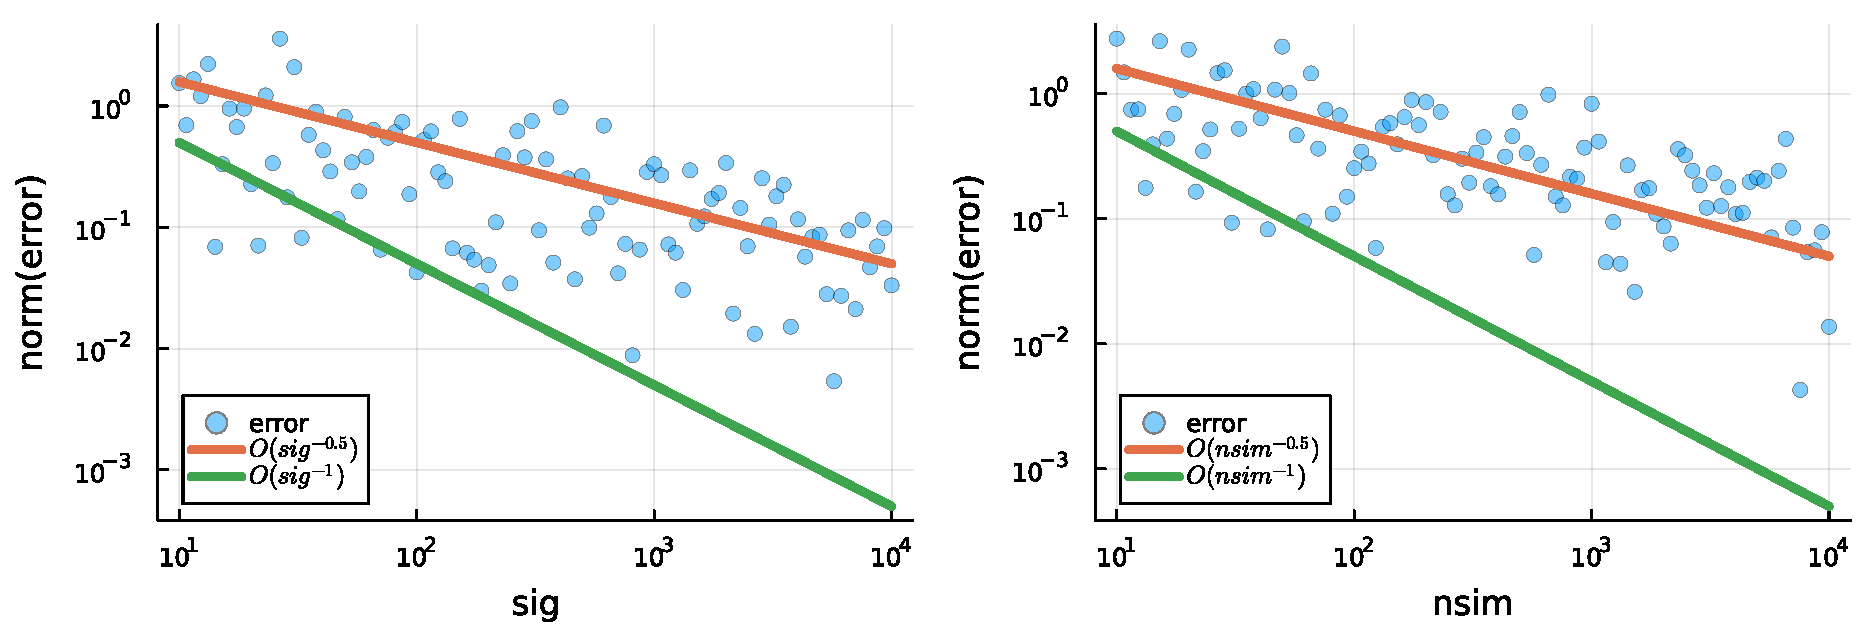
\includegraphics[width=\textwidth]{imgs/convergence_main_poisson.pdf}
        \caption{Realizaties van de norm van de fout,
            met $nsim =1$ en $\sigma$ variabel of $nsim$ variabel en $\sigma = 1$.
            Hoeveelheid samples van $A$ per simulatie $= \text{Poisson}(\sigma)$.
        }
        \label{fig:imgs/main poisson convergentie}
    \end{figure}
\end{frame}

\begin{frame}
    \frametitle{Main Poisson algoritme (opmerkingen)}
    \begin{equation}
        y(t) \cong Y(t) =  \prod_{k=1}^{N_{t}}\left(I + \frac{A(T_{k})}{\sigma} \right)    y(0).
    \end{equation}
    \begin{itemize}
        \item TB: $E[Y(t)],Var[Y(t)]< \infty$
        \item Parallelle complexiteit
        \item Volgorde matrix vermenigvuldingen $v^{T}y(t)$
        \item Inspiratie uit \cite{acebron_monte_2016}
    \end{itemize}
\end{frame}

\section{Geavanceerde methoden}

\section{Conclusie}

\begin{frame}
    \frametitle{Limitaties}
    \begin{itemize}
        \item Stabiliteit $\rightarrow$ \cite{kettunen_unbiased_2021}
              (efficiënte unbiased $e^{\int A(s) ds } y(0)$ )
        \item Biased voor non-lineaire ODEs
    \end{itemize}
\end{frame}

\begin{frame}
    \frametitle{Toekomstig Werk}
    \begin{itemize}
        \item Random ODEs
        \item Specifieke ODEs
    \end{itemize}
\end{frame}

% 6 min
% \begin{frame}
%     \frametitle{Unbiased Non-Linearity}
%     \begin{itemize}
%         \item exponentiele voorbeeld + screenshot paper
%         \item VRE
%         \item Feynman-Kac formule
%         \item Magnus series
%     \end{itemize}
% \end{frame}

\end{document}